\documentclass[12pt]{article}
\usepackage[usenames]{color} %used for font color
\usepackage{amssymb} %maths
\usepackage{amsmath} %maths
\usepackage{graphicx}

\newcommand{\GeV}{\ensuremath{\mathrm{GeV}}}
\newcommand{\TeV}{\ensuremath{\mathrm{TeV}}}
\newcommand{\GeVc}{\ensuremath{\mathrm{GeV}}}
\newcommand{\TeVc}{\ensuremath{\mathrm{TeV}}}
\newcommand{\GeVcc}{\ensuremath{\mathrm{GeV}}}
\newcommand{\TeVcc}{\ensuremath{\mathrm{TeV}}}
\newcommand{\pt}            {\ensuremath{p_{\mathrm{T}}}\xspace}
\newcommand{\kt}            {\ensuremath{k_{\mathrm{T}}}\xspace}
\newcommand{\antikt}        {anti-\kt}
\newcommand{\ttbar}        {\ensuremath{\mathrm{t}\overline{\mathrm{t}}}}
\newcommand{\bbbar}        {\ensuremath{\mathrm{b}\overline{\mathrm{b}}}}
\newcommand{\qqbar}        {\ensuremath{\mathrm{q}\overline{\mathrm{q}}}}
\newcommand{\fbinv}        {\ensuremath{\mathrm{fb}^{-1}}}
\newcommand{\instlumiA}     {\ensuremath{\times 10^{33} \mathrm{cm}^{-2} \mathrm{s}^{-1}}}
\newcommand{\instlumiB}     {\ensuremath{\times 10^{34} \mathrm{cm}^{-2} \mathrm{s}^{-1}}}

\begin{document}

\title{Exascale Computing at the LHC : Narrative}
\author{Matthew Jones, Steven Ko, Salvatore Rappoccio, Lukasz Zialek}

\maketitle

\clearpage

\section{Funding Strategy}

Exascale computing is an enormously growth-oriented area. Even during
lean economic times, the US Federal Government is pledging to support
this area of research, for instance in the Department of Energy
Exascale Computing Initiative~\cite{doe_eci}. Indeed, the DOE Office of
Science has this to say about the area:
\begin{quote}
The Exascale initiative will be significant and transformative for Department of Energy missions.
\end{quote}
The current level of funding for the DOE EIC and related activities is
\$21M.~\cite{doe_eci_budget}. 

In addition to governmental programs such as above, private sector
funding sources are also available, such as the Google Faculty
Research Awards~\cite{google_fac_awards}, which has an interest in
exascale computing projects also. 

\bigskip

{\bf Need more bla bla bla}. 

\clearpage

\section{Project Organization}

The principle investigators (PIs) of this proposal have a
widely-varied and applicable skill set to accomplish the goals of
extending LHC computing to the exascale. 

\begin{itemize}
\item Salvatore Rappoccio has 15 years of experience programming in a
high-energy physics environment, as well as other numerical software
design for the private sector. He is an expert in several critical
areas of event reconstruction at CMS which can be optimized for
multicore usage. 
\item Lukasz Ziarek \ldots. 
\item Steven Ko \ldots. 
\item Peter Elmer \ldots.  
\item Matthew Jones \ldots.  
\end{itemize}




\bigskip

{\bf Add your bla bla bla above. }. 


\clearpage

\section{Introduction}

With the discovery of a new boson with mass around $m=125$
\GeV ~\cite{higgs_cms,higgs_atlas} (henceforth referred to as the
$H$), a new phase of particle physics
has begun. The questions have shifted from the cause of the breaking
of the electroweak symmetry, to the nature of that symmetry
breaking. Two major questions arise. The first is the exact nature of
the particle responsible for the electroweak symmetry breaking. The
second is how a particle with a relatively low mass around $m=125$ \GeV\ 
can be responsible for electroweak symmetry breaking 
without extremely large fine tuning in nature, cancelling
the large radiative corrections to its mass. 

With 25 $\fbinv$ of 7 and 8 \TeV data delivered by the LHC in
2011-2012, and instantaneous luminosities reaching
$7\instlumiA$, the processing
time to reconstruct each event collected by CMS was approximately 20
seconds per event. However, as the instantaneous luminosity is
increased, the computational time currently scales quadratically. As
the upgraded LHC is expected to deliver $>12\instlumiA$ in the
upcoming run, the processing time per event is expected to reach
several minutes per event as shown in
Figure~\ref{lumitpeSingleMu}. Furthermore, in future runs of the LHC
in the next 15 years, the luminosity is expected to reach as high as
$>1\instlumiB$, which would correspond (naively) to several hours of
computational time per event! Clearly, it is necessary for the
computing power to scale in order to compensate for this dramatic
increase in CPU time with instantaneous luminosity. 


However, with the expected end of the historic scaling of single-core
processing capability~\cite{bergman2008exascale} ({\bf NEED MORE
  MATERIAL HERE}), it is imperative to utilize a parallel processing
strategy in order to maintain the levels of computational speed of LHC
data in the immediate future. 


\bigskip

{\bf Need more bla bla bla}. 



\begin{figure}[h!]
    \centering
    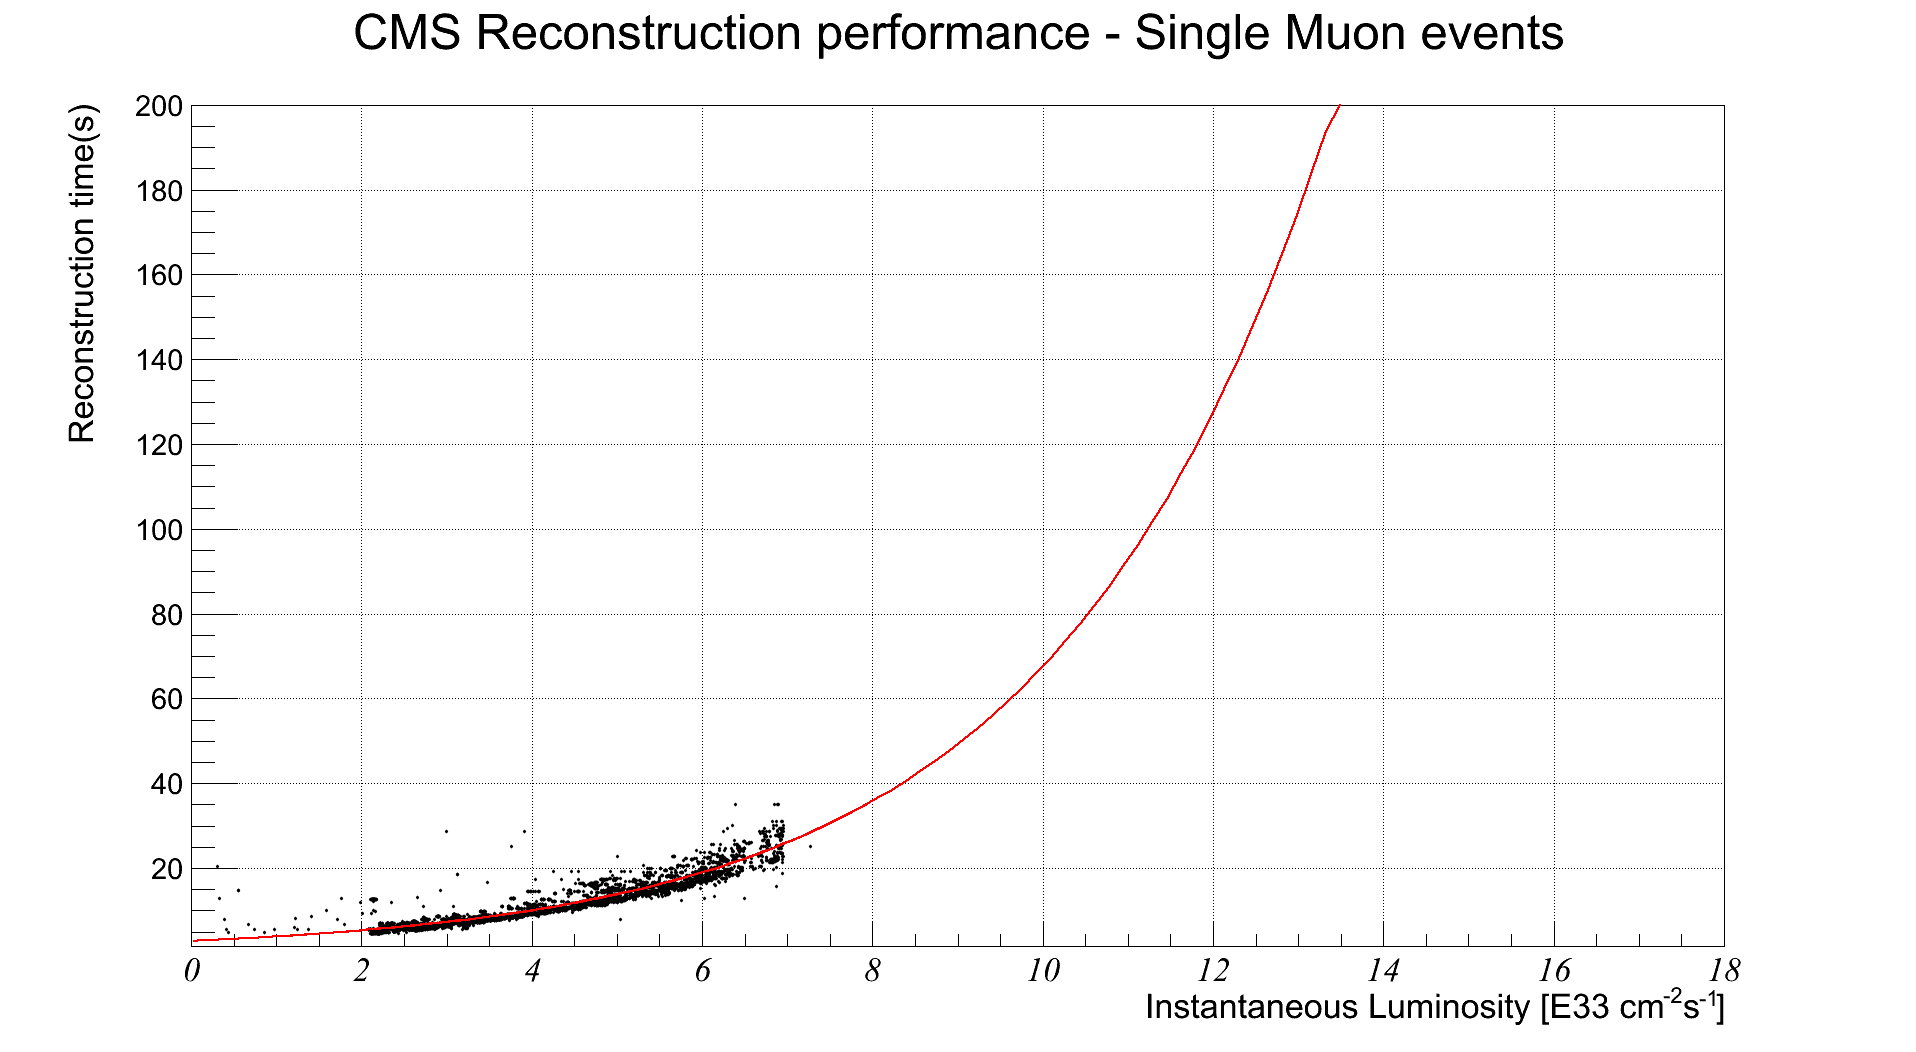
\includegraphics[width=100mm]{lumitpeSingleMu-fitted2.png}
    \caption{\label{lumitpeSingleMu} Event processing time versus
      instantaneous luminosity.}
\end{figure}

\bibliographystyle{h-elsevier}
\bibliography{collaborative_proposal}{}
%\bibliography{auto_generated}

\end{document}
